\documentclass[12pt]{article}
\usepackage{amsmath}
\usepackage{graphicx}
\usepackage{hyperref}
\usepackage[ngerman]{babel}
\setlength\parindent{0pt}
\graphicspath{ {./img/} } 
\usepackage{amsfonts}
\usepackage{tikz}
\hypersetup{pdfborder=0 0 0}

\title{Algorithmen und Komplexität Zusammenfassung}
\author{Fabian Sigmund}
\date{11.07.2023}



\tikzset{
	heap/.style={
		every node/.style={circle,draw},
		level 1/.style={sibling distance=70mm},
		level 2/.style={sibling distance=70mm}
	}
}


\begin{document}
	\maketitle
	\pagebreak
	\tableofcontents
	\pagebreak
	\section{Sortieralgorithmen (Einfach)}
	
	Im folgenden gilt:
	\newline
	n: Anzahl der Elemente im Array\newline
	$\lambda$: Vertausch-Operationen \newline
	$\mu$: Vergleichs-Operationen
	
	\subsection{Selection Sort}
	
	\begin{itemize}
		\item Prinzip: Vertausche kleinstes Element der unsortierten Liste mit ihrem ersten Elemen
		\item Zeit-ineffizient: Andere Elemente bleiben unberührt
		\item Platz-effizient: Dreieckstausch zwischen erstem und kleinstem Element
		\item einfach zu implementieren
		\item In-place, Instabil, $ \mathcal{O}(n^2) $ 
	\end{itemize}
	
	\textbf{a) Sortieren Beispiel:}
	
	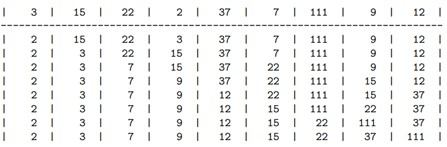
\includegraphics{SelectionSort}
	\break
	
	\textbf{b) Vertausch-Operationen ($\lambda$)} \hfill \break
	
	\begin{center}
		$\lambda = n - 1$
	\end{center}
	
	Anmerkung: Selbstvertauschung tritt auf, wenn das jetzige Element schon an der richtigen Stelle ist. Diese müssen per Hand aus der Tabelle von a) ausgelesen werden.

		\pagebreak
	\textbf{c) Vergleichs-Operationen ($\mu$)}
	\newline
	\newline
	
	
	\begin{center}
		$\mu = $\Large{$\frac{n(n-1)}{2}$}
	\end{center}
	
	Anmerkung: Egal nach welchem Kriterium sortiert wird, diese Formel gilt immer!
	
	\pagebreak
	
	
	\subsection{Insertion Sort}
	
	\begin{itemize}
		\item Prinzip: Füge Elemente der Reihe nach an richtiger Position ein
		\item Zeit-ineffizient:
			\subitem Für jede Einfüge-Operation wird gesamte Liste durchlaufen
			\subitem Im Array müssen alle folgenden Element verschoben werden
		\item Platz-effizient: Nur ein Element als Zwischenspeicher
		\item einfach zu implementieren
		\item In-place, Stabil, $ \mathcal{O}(n^2) $ 
		
	\end{itemize}
	\textbf{a) Sortieren Beispiel}
	
	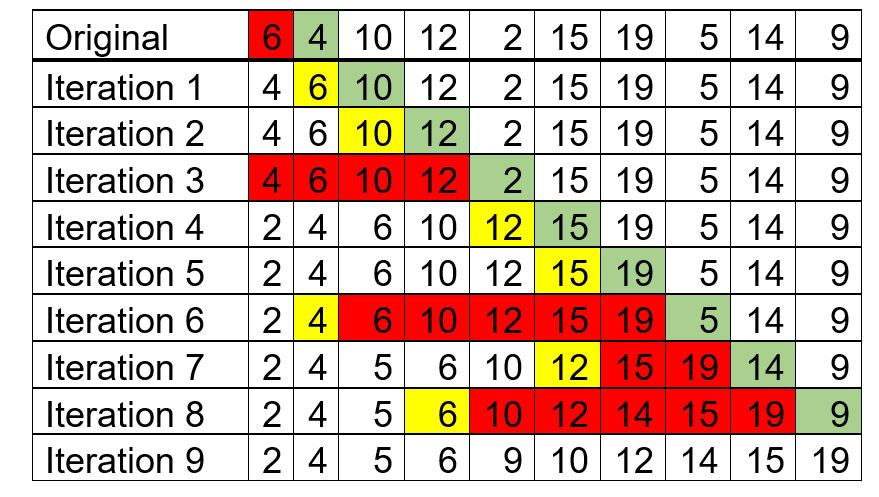
\includegraphics[scale=0.5]{InsertionSort}
	\hfill \break
	
	\textbf{b) Vertausch-Operationen ($\lambda$)} \hfill \break
	
	1.	Markiere in jeder Zeile die „Vergleichs-Diagonale grün“
	
	2.	Markiere in jeder Zeile rot bis zum Index auf das grün markierte Element
	
	3.	Vertausch-Operationen = Anzahl der roten Elemente\hfill \break
	
	\textbf{c) Vergleichsoperationen ($\mu$)} \hfill \break
	
	1.	Schritte 1 und 2 von „Vertausch-Operationen“
	
	2.	Markiere, wenn möglich, links ein zusätzliches Kästchen gelb
	
	3.	$\mu$ = Anzahl der roten Elemente + Anzahl der gelben Elemente
	
	\newpage
	
	\subsection{Bubble Sort}
	\begin{itemize}
		\item Prinzip: Nach jeder Iteration "bubbelt" das größte Element auf die richtige Stelle
		\item Zeit-ineffizient:Große Elemente werden zunächst relativ schnell richtig am Ende einer Liste einsortiert. Kleinere Elemente werden jedoch nur eher langsam nach vorn verschoben
		\item Platz-Effizienz: Dreieckstausch zwischen den größten und nachfolgenden Elemente
		\item einfach zu implementieren 
		\item In-place, Stabil, $ \mathcal{O}(n^2) $ 
	\end{itemize}
	\textbf{a) Sortieren Beispiel}
	\newline\newline
	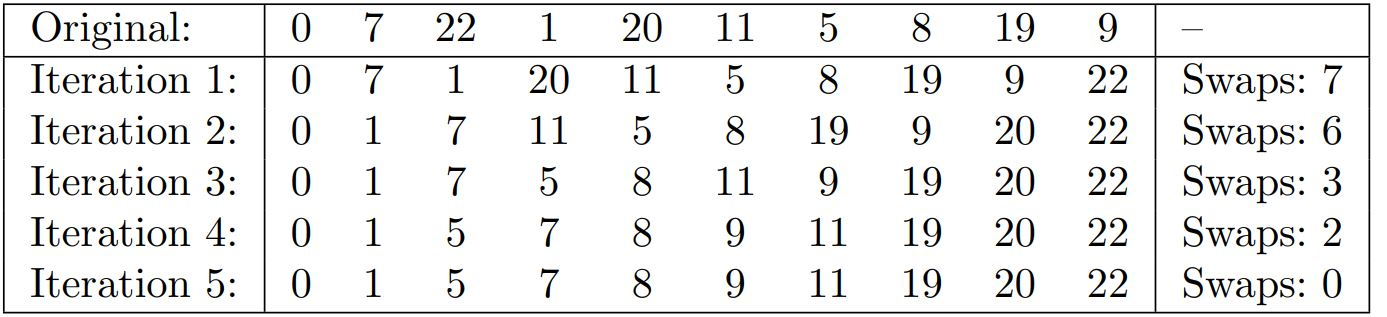
\includegraphics[scale=0.5]{BubbleSort}
	\newline
	
	\textbf{b) Vertausch-Operationen ($\lambda$)} \hfill \break
	
	Kein Muster, nur doch durchzählen möglich. \hfill \break
	\newline
	\textbf{c) Vergleichsoperationen ($\mu$)}
	

		\begin{center}
		$\mu = selbst geschrieben \ Zeilen * Elemente$
	\end{center}
\newpage
\section{Sortieralgorithmen Divide and Conquer}
\subsection{QuickSort}
\begin{center}
	Original:
\end{center}
\vspace{-0.8cm}
 \begin{center}
 	

 [ 3, 8, 17, 5, 15, 2, 1, 12, 4, 9 ]
 \end{center}
1. Pivotelement wählen und mit dem letzten Element tauschen.
 \begin{center}
	[ 9, 8, 17, 5, 15, 2, 1, 12, 4, (3) ]
\end{center}
2. Von \textbf{links} ausgehend Element suchen, das \textbf{größer} ist als das Pivotelement.

 \begin{center}
	[ \textbf{9}, 8, 17, 5, 15, 2, 1, 12, 4, (3) ]
\end{center}

3. Von \textbf{rechts} ausgehend Element suchen, das \textbf{kleiner} ist als das Pivotelement.

\begin{center}
	[ 9 , 8, 17, 5, 15, 2, \textbf{1}, 12, 4, (3) ]
\end{center}




4. Elemente aus 2. und 3. tauschen
\begin{center}
	[ \textbf{1}, 8, 17, 5, 15, 2, \textbf{9}, 12, 4, (3) ]
\end{center}

5. Schritt 2-4 solange wiederholen bis der Index des Elements aus 2. größer ist als der Index des Elements aus 3.

\begin{center}
	[ \textbf{1}, \textbf{2}, 17, 5, 15, \textbf{8}, \textbf{9}, 12, 4, (3) ]
\end{center}

6. Pivot Element an die richtige stelle zurücktauschen.

\begin{center}
	[ 1, 2, (3), 5, 15, 8 , 9, 12, 4, 17 ]
\end{center}

7. Liste am Pivot Element aufspalten

\begin{center}
	[ 1, 2 ] (3) [ 5, 15, 8 , 9, 12, 4, 17 ]
\end{center}

8. Schritte 1-7 wiederholen bis Liste sortiert ist.
	[(1),  [2]] (3) [4, (5), ]
\newpage

\subsection{Mergesort}
\subsubsection{TopDown (Rekursiv)}
\begin{center}
	$Aufrufe \ mit \ initialen \ Aufruf = \Large{2n-1}$
\end{center}

\subsubsection{BottomDown (Iterativ)}
\begin{center}
	$Iterationen \ der \ \ddot{a}ußeren \ Schleife =  \lceil \log_{2} n \rceil $
\end{center}
\newpage

\section{Sortieren Zusammenfassung}

\textbf{Einfache Verfahren}

\begin{itemize}
	\item vergleichen jedes Paar von Elementen
 	\item bearbeiten in jedem Durchlauf nur ein Element
	 \item verbessern nicht die Position der anderen Elemente
	\item $ \mathcal{O}(n^2) $ 
\end{itemize}
\textbf{Effiziente Verfahren}
\begin{itemize}
	\item Unterschiedliche Ansatze: 
	\subitem erst grob, dann fein: Quicksort
	\subitem erst im Kleinen, dann im Großen: Mergesort
	\subitem spezielle Datenstruktur: Heapsort
	\item Effizienzgewinn durch
	\subitem Vermeidung unnotiger Vergleiche
	\subitem effiziente Nutzung der in einem Durchlauf gesammelten Infos
	\subitem Verbessern der Position mehrerer Elemente in einem Durchlauf
	\item $ \mathcal{O}(n\log n) $  (as good as it gets)
\end{itemize}

\section{Komplexitätsklassen}

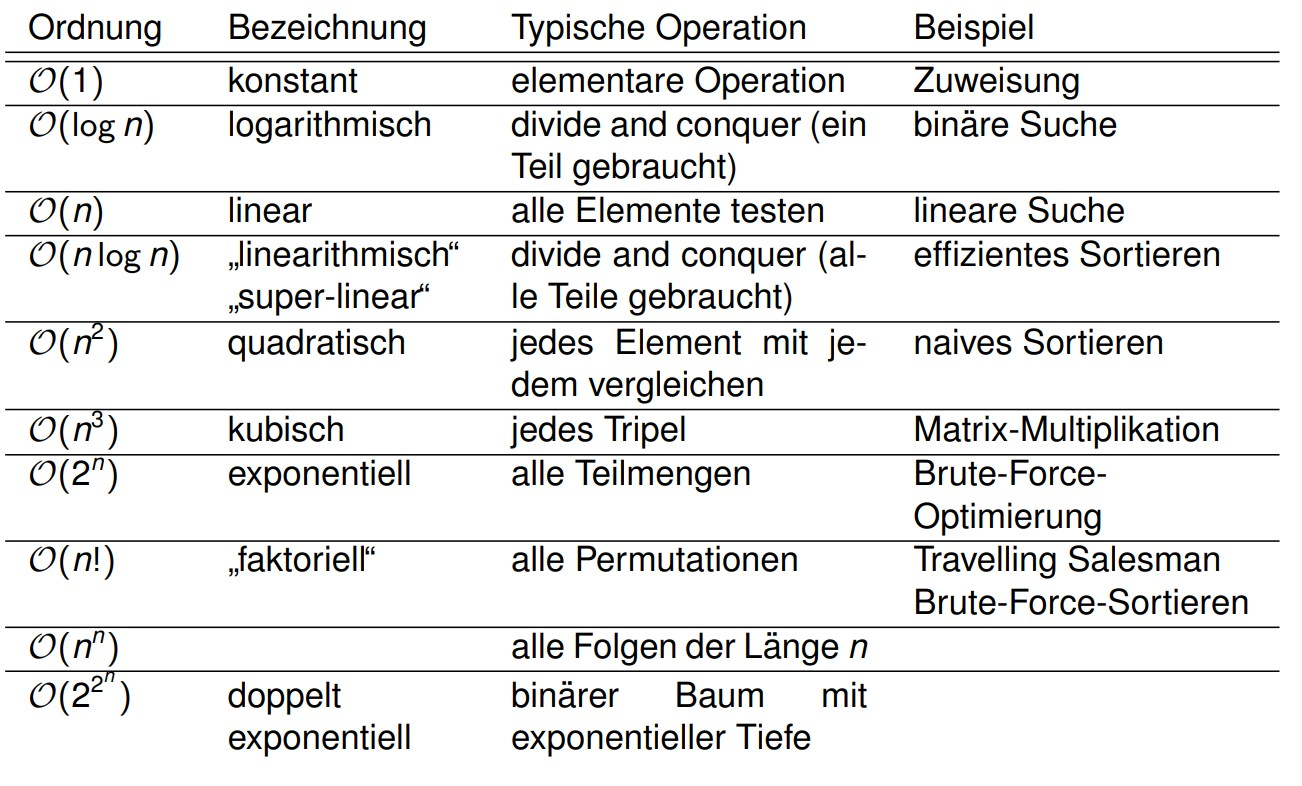
\includegraphics[scale=0.4]{KK}

\subsection{$\mathcal{O}$-Notation und Landau-Symbole}

g wächst höchstens so schnell wie f: \newline
 $ g \in \mathcal{O}(f): \lim \limits_{x \to \infty} \frac{g(x)}{f(x)} = c \in \mathbb{R} $ \hfill \break

g wächst mindestens so schnell wie f:\newline
 $ g \in\Omega(f): \lim \limits_{x \to \infty} \frac{f(x)}{g(x)} = c \in \mathbb{R} $ \hfill \break
 

g wächst genau so schnell wie f bis auf einen konstanten Faktor:\newline
$ g \in \theta (f): \lim \limits_{x \to \infty} \frac{g(x)}{f(x)} = c \in \mathbb{R}^{>0} $ \hfill \break



g wächst genau so schnell wie f: \newline
$ g \sim f: \lim \limits_{x \to \infty} \frac{f(x)}{g(x)} = 1 $ \hfill \break

\subsection{Master-Theorem}

\includegraphics{Master}
\newpage
\section{Bäume}





\subsection{Heaps}

\textbf{Definition: Heap}
Ein (binarer) Heap ist ein (fast) vollständiger binärer Baum, in dem für jeden Knoten gilt, dass er in einer definierten Ordnungsrelation zu seinen Nachfolgern steht.
\begin{itemize}
	\item Max-Heap: Jeder Knoten ist $ \geq $ als seine Nachfolger
	\item Min-Heap: Jeder Knoten ist $ \leq $ als seine Nachfolger
\end{itemize}

Fast vollständiger Binärbaum:
\begin{itemize}
	\item Alle Ebenen bis auf die unterste sind vollständig
	\item Die unterste Ebene ist von links durchgehend besetzt
\end{itemize}

\subsubsection{Wichtige Operationen auf Heaps}

\textbf{Im folgenden Beispiel anhand von Max-Heaps, für Min-Heaps gelten die Aussagen analog}
\newline

\textbf{heapify}: Stelle die Heap-Eigenschaft eines fast vollständigen Binärbaums her 
\begin{itemize}
	\item bubble up: Lasse einen großen Knoten nach oben steigen
	\item bubble down: Lasse einen kleinen Knoten nach unten sinken
\end{itemize}
\textbf{insert}: Füge ein neues Element in den Heap ein \newline
\newline




\begin{tikzpicture}[heap, sibling distance=70mm]
	\node {12}
	child{node{6}
		child{node{3} 
			child{node{5}
				child{node{4}}
			 } 
		child{node{7}}
		 }
	child{node{16}}
}	
	;
	
	
\end{tikzpicture}

\begin{tikzpicture}[heap]
	\node {7}
	child{node{12}
		child{node{25}} child{node{14}}}
	child{node{9}}
	;
\end{tikzpicture}
\newpage
\subsection{Binäre Suchbäume}

\textbf{Definition: Binärer Suchbaum} \newline
Eine Binärer Suchbaum ist ein Binärbaum mit folgenden Eigenschaften:
\begin{itemize}
	\item Die Knoten des Baums sind mit Schlüsseln aus einer geordneten Menge K beschriftet
	\item Für jeden Knoten N gilt:
	\subitem \small{Alle Schlüssel im linken Teilbaum von N sind kleiner als der Schlüssel von N}
	\subitem \small{Alle Schlüssel im rechten Teilbaum von N sind größer als der Schlüssel von N}
\end{itemize}

\subsubsection{Wichtige Operationen auf binären Suchbäumen}

\textbf{insert}:
\begin{itemize}
	\item Suche nach \textit{K}
	\item Falls \textit{K} nicht im Baum ist, setze es an der Stelle ein, an der es gefunden worden wäre
\end{itemize}


\textbf{delete}:
Fallunterscheidung:
\begin{itemize}
	\item Fall 1: Knoten \textit{K} hat keinen Nachfolger
	\subitem Lösung: Schneide Knoten ab
	\item Fall 2: Knoten \textit{K} hat einen Nachfolger
	\subitem Lösung: Ersetze Knoten durch seinen einzigen Nachfolger
	\item Fall 3: Knoten \textit{K} hat zwei Nachfolger
	\subitem Suche größten Knoten \textit{G} im linken Teilbaum
	\subitem Tausche \textit{G} und \textit{K}
	\subitem Lösche \textit{K} im linken Teilbaum von (nun) G
\end{itemize}
\newpage
\subsection{AVL-Bäume}


\end{document}
